\documentclass[tikz,border=10pt]{standalone}
\usepackage{amsmath}
\usepackage{tikz}
\usetikzlibrary{positioning}

\tikzset{
  card/.style={draw=blue!70!black, line width=1.2pt, rounded corners=3pt, minimum width=5.5cm, minimum height=4.2cm, align=left, fill=none},
  note/.style={font=\small, align=left}
}

\begin{document}
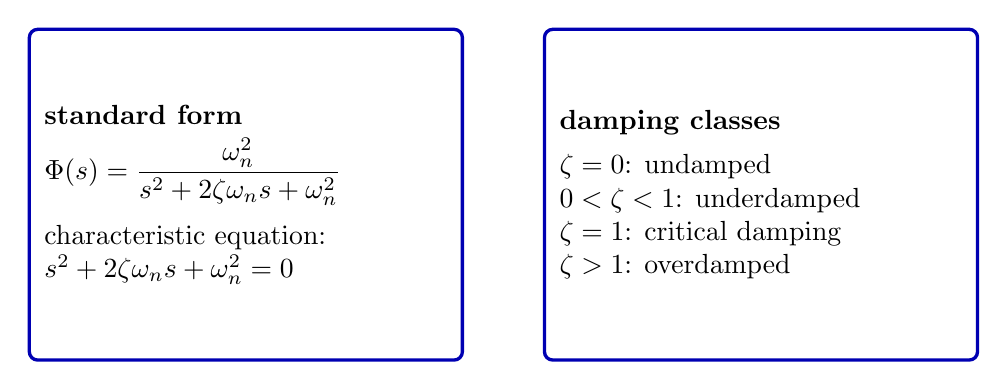
\begin{tikzpicture}[node distance=0.9cm]
  \node[card] (left) {
    \begin{minipage}{5.0cm}
      \textbf{standard form}\\[4pt]
      $\Phi(s)=\dfrac{\omega_n^2}{s^2+2\zeta\omega_n s+\omega_n^2}$\\[6pt]
      characteristic equation:\\
      $s^2+2\zeta\omega_n s+\omega_n^2=0$
    \end{minipage}
  };
  \node[card, right=1.0cm of left] (right) {
    \begin{minipage}{5.0cm}
      \textbf{damping classes}\\[4pt]
      $\zeta=0$: undamped\\
      $0<\zeta<1$: underdamped\\
      $\zeta=1$: critical damping\\
      $\zeta>1$: overdamped
    \end{minipage}
  };
\end{tikzpicture}
\end{document}
